%!TEX root = ../main.tex

Le deuxième chapitre de ce mémoire décrira les différentes techniques utilisées par les virus 
dans le processus d'infection, ainsi que les techniques employées par ces derniers pour dissimuler leurs présences.
%vérifié

Ce chapitre portera aussi sur différentes notions qui ont une relation plus ou moins indirecte avec les virus,
et qui sont nécessaires pour la réalisation d'une étude plus propre et plus claire. %vérifié

\newpage

\section{Les virus} 
Un virus informatique est un programme parasite généralement de petite taille, 
doté d’une capacité d’infection et de multiplication, et possède une fonction nocive appelée 
\emph{Payload}\footnote{Le terme Payload (charge utile en français) au figuré pour désigner 
la partie du code exécutable d'un virus qui est spécifiquement destinée à nuire.}.

La fonction d'infection permet au virus de s'introduire dans des fichiers de programme, 
dans des fichiers de données utilisant un langage de script ou dans le secteur de démarrage 
d’un disque dur. Lors de l'accès à ces programmes ou secteur, le code du virus s'exécutera de 
façon d'abord silencieuse (phase de multiplication pendant laquelle il infectera d'autres fichiers) 
puis visible (activation de la fonction nocive). %vérifié

La fonction nocive pourra être déclenchée par un événement particulier, elle peut se limiter 
à l'affichage d'un message agaçant ou, plus généralement, conduire à des perturbations graves 
de l'ordinateur comme des ralentissements du fonctionnement, effacement ou corruption de 
fichiers ou pire encore le formatage du disque dur. \cite{virus_informatique} %vérifié

Les virus peuvent se propager d'une machine a une autre par biais des périphérique de stockage comme les disquettes, 
les CD-ROM ou les clé USB.

Ci-dessous se trouve un pseudo code exemple d'un virus informatique :
\begin{verbatim}
    def virus():
        infecter()
        if gachette() is True:
            executer_charge()
\end{verbatim}


\section{Classification des virus par cible}
L'un des moyens de classifications des virus est de voir ce qu'ils essayent d'infecter.
Dans cette section, trois classes de virus seront abordées : les virus visant les programmes, les virus système,
et les virus interprétés. %vérifié

    \subsection{Virus visant les programmes}
    Les virus qui visent les programmes, cherchent à infecter les exécutables binaires compilés. 
    Le principe de fonctionnement est le suivant : le virus est présent dans un fichier exécutable, lorsque 
    ce dernier est exécuté, le virus choisit et contamine un ou plusieurs autres fichiers ; si le virus se maintient
    en mémoire, il infecte d'autres fichiers à l'exécution, ou simplement lors d'une manipulation. 
    \cite{virus_informatique_article}%vérifié

    Il existe plusieurs types de programmes, et chacun d'eux peut faire l'objet d'une attaque virale spécifique 
    \cite{virus_informatique_article} : %vérifié
    \begin{description}
        \item[Programmes DOS :] Jusqu’en 1999, la majorité des virus visant les programmes fonctionnaient sous 
            DOS et ciblaient les fichiers exécutables par ce système d'exploitation. 
            Déjà limitée à cette époque, la proportion des infections dues à ces virus DOS n’a cessé 
            de diminuer pour être presque inexistante aujourd’hui. %vérifié
        \item[Applications Windows 16 bits :] Ces programmes sont aussi appelés \emph{New Executable} (NE).
            Ils sont rencontrés dans les environnements \emph{Windows 3.x}. %vérifié

        \item[Applications Windows 32/64 bits :] Ces programmes sont aussi appelés \emph{Portable Executable}
            (PE). Ils sont rencontrés dans les environnements \emph{Windows actuels}.%vérifié

    \end{description}

    \subsection{Virus système}
    Pour une meilleure compréhension de cette section, il est indispensable d'expliquer la procédure 
    de démarrage des ordinateurs. Bien que la procédure de démarrage diffère d'une machine à une autre, 
    la démarche générale reste la même : \cite{virus} %vérifié
    \begin{enumerate}
        \item Allumage. %vérifié
        \item Les instructions de la ROM sont exécutées  avec un auto-test, détection de périphérique et 
            initialisation. Le périphérique de démarrage est identifié et le secteur de démarrage est 
            lu de ce dernier. Une fois cette action accomplie, le contrôle est transféré au code chargé. 
            Cette étape est appelée le démarrage primaire. %vérifié
        \item Le code chargé durant le démarrage primaire, charge un programme encore plus grand et plus sophistiqué 
            qui comprend la structure des systèmes de fichiers et lui donne le contrôle. Cette étape est appelée
            le démarrage secondaire. %vérifié
        \item Le démarrage secondaire charge et exécute le noyau du système d'exploitation. %vérifié
    \end{enumerate}
    
    Un virus appartenant à cette classe infecte en se copiant dans le secteur de démarrage. Puis il copie le contenu du secteur de démarrage dans un autre emplacement sur le disque dur  pour que le virus 
    puisse lui transférer le contrôle afin que la  procédure de démarrage continue normalement.
    \cite{virus} %vérifié

    Le problème qui peut se poser avec la préservation du secteur de démarrage, est que l'allocation d'un secteur 
    sur le disque diffère d'un système de fichier à un autre. Allouer proprement un espace pour sauvegarder 
    le secteur de démarrage nécessite beaucoup de code, ce qui n'est pas possible, car le code des virus
    appartenant à cette classe doit être court à cause de la taille limitée des secteurs de démarrage.
    Une solution à ce problème consiste à toujours sauvegarder le secteur de démarrage dans un endroit fixe et sûr.
    Mais cette solution alternative peut poser un problème si une machine est infectée par plusieurs virus qui utilisent
    le même endroit pour sauvegarder le secteur de démarrage, car un virus peut facilement détruire complètement 
    le code de démarrage en l'écrasant avec le code d'un autre virus de même classe. \cite{virus} %vérifié

    Malgré les problèmes présentés ci-dessus, infecté le secteur de démarrage est une stratégie qui donne beaucoup
    d'avantages au virus. Même si la position du virus est connue, ce dernier s'exécute avant même que le système 
    d'exploitation ou l'anti-virus procède au démarrage ; ce qui lui permet de bien se cacher en désactivant les mesures 
    de sécurité avant leurs démarrages. %vérifié


    Les virus de cette classe sont rares maintenant, car la majorité des systèmes d'exploitation interdit l'écriture
    sur les secteurs de démarrage sans des autorisations bien précises.

    \subsection{Virus interprété}
    Cette classe de virus regroupent principalement les virus macro et les virus script. %vérifié
        \subsubsection{Virus macro}
        Du fait de la sophistication des outils de bureautique actuels, tout fichier de données doit être 
        considéré comme potentiellement dangereux. Même si aujourd’hui de nombreux standards de fichier 
        n’acceptent pas l’encapsulation de routines automatisables (macros ou scripts), 
        cette technique tend à se développer. Un type de fichier aujourd’hui inoffensif pourra ainsi 
        rapidement devenir dangereux. \cite{virus_informatique_article} %vérifié

        Jusqu’à l’arrivée de WM/Concept\footnote{Le WM/Concept est le premier macro-virus largement connu
        développé pour \emph{Microsoft Word 6.}} en 1995, le grand public était persuadé qu’un virus, 
        considéré à juste titre comme un programme, ne pouvait être véhiculé et introduit dans un ordinateur 
        qu’avec l'aide éventuelle d’un autre programme. En clair, seuls les fichiers exécutables ou les zones 
        systèmes des disquettes pouvaient, après infection, propager à leur tour le virus. 
        A contrario, les fichiers ne contenant que des données étaient sans danger. \cite{virus_informatique_article}
        %vérifié

        La sophistication des outils de bureautiques avec l’apparition des langages de macro a bouleversé 
        la donne. Sans toujours en imaginer les conséquences, les fichiers de données contenant textes ou feuilles 
        de calcul se sont trouvés enrichis de routines automatisables et programmables. 
        Par là même, ils devenaient un nouveau terrain de jeux pour les auteurs de virus. 
        \cite{virus_informatique_article} %vérifié


        \subsubsection{Virus script}
        Un langage de script est un langage de programmation spécialisé destiné à contrôler l'environnement 
        d'un logiciel. Interprété, il peut donc être exécuté sur toute machine disposant de l'interpréteur approprié. 
        \cite{virus_informatique_article} %vérifié

        Donc, un virus de script est un virus écrit dans un langage interprété, et qui utilise l'interpréteur approprié
        pour exécuter sa charge virale et infecter d'autres scripts. %vérifié

\section{Classification des virus par techniques de dissimulations}
Une autre manière de classer les virus est par la façon dont ils essaient de se cacher, 
à la fois des utilisateurs et des logiciels anti-virus. \cite{virus} %vérifié

    \subsection{Aucune dissimulation}
    Le virus n'essaye pas de cacher sa présence ou son code, il réagit plutôt comme un exécutable ordinaire. %vérifié

    \subsection{Chiffrement}
    L'idée est de chiffrer le corps du virus (infection, gâchette, et charge) pour le rendre plus difficile à 
    détecter. Ce chiffrement n'est pas ce qu'appellent les cryptographes un cryptage, mais plutôt un moyen pour
    brouiller la tâche de détection. \cite{virus} %vérifié

    Par ailleurs si le code du virus est chiffré, il ne peut être exécuter. Pour régler ce problème, une boucle 
    de déchiffrement le précède. Celle ci sera exécuter en premier au lancement du virus, pour déchiffrer le 
    corps de ce dernier. Le principe est que la boucle de chiffrement est petite par rapport au corps du virus, 
    ce qui la rend plus difficile à détecter par les anti-virus. \cite{virus} %vérifié

    Les virus utilisent plusieurs méthodes pour chiffrer leurs corps, on y trouve : \cite{virus} %vérifié
    \begin{description}
        \item[Chiffrement simple :] Aucune clé n'est utilisée, juste l'utilisation d'opérations basiques comme
            l'incrémentation, la décrémentation, le décalage \ldots{} Exemple :
            \begin{center}
            \begin{tabular}{cc}
                \toprule
                Chiffrement & Déchiffrement \\
                \midrule
                inc corps[i] & dec corps[i] \\
                rol corps[i] & ror corps[i] \\
                \bottomrule
            \end{tabular}
            \end{center}

        \item[Chiffrement statique :] Une clé statique et constante est utilisée pour le chiffrement. Les opérations
            qui peuvent être utilisées sont les opérations arithmétiques comme l'addition, et les opérations logiques
            comme le \emph{xor}\footnote{Le \emph{xor} est l'opération \emph{ou exclusive}.}. %vérifié
            \begin{center}
            \begin{tabular}{cc}
                \toprule
                Chiffrement & Déchiffrement \\
                \midrule
                corps[i] + 45 & corps[i] - 45\\
                corps[i] xor 13 & corps[i] xor 13 \\
                \bottomrule
            \end{tabular}
            \end{center}

        \item[Chiffrement variable :] La clé commence comme une valeur constante, puis change avec 
            la procédure de déchiffrement. Exemple : %vérifié
            \begin{verbatim}
                cle = 354
                for i in 0..longueur(corps):
                    corps[i] = corps[i] xor cle
                    cle += corps[i]
            \end{verbatim}

    \end{description}
    Le point faible majeur du chiffrement est que le corps du virus reste le même d'une infection à une autre. Ainsi, 
    détecter une seule infection de ce virus suffit pour détecter toutes les autres infections. \cite{virus} %vérifié

    Une technique pour contourner ce problème consiste à changer la clé de chiffrement d'une infection à une autre, ce
    qui permet au virus d'avoir un corps (chiffré) différent à chaque infection. \cite{virus} %vérifié

    \subsection{Furtivité}
    Un virus furtif est un virus qui cache non seulement son corps, mais également l'infection elle-même,
    en prenant régulièrement des mesures pour y arriver. 
    Un exemple simple d'une technique de furtivité consiste à restaurer la date de modification d'un fichier infecté.
    %vérifié

    \subsection{Oligomorphisme}
    En supposant que la clé de chiffrement est modifiée avec chaque infection, la seule partie qui ne change pas
    dans le virus est la boucle de déchiffrement. Donc, un anti-virus peut exploiter ce fait pour détecter le virus. 
    \cite{virus} %vérifié

    Un virus oligomorphe est un virus chiffré qui a dans la poche un nombre limité (dizaines ou centaines) 
    de boucles de déchiffrement. Le virus sélectionne une nouvelle boucle de déchiffrement 
    pour chaque nouvelle infection. \cite{virus} %vérifié

    En terme de détection, l'oligomorphisme rend le virus un petit peu plus difficile à repérer. Au lieu de chercher
    une seule boucle de déchiffrement, l'anti-virus doit chercher toutes les variantes. \cite{virus} %vérifié

    \subsection{Polymorphisme}
    Un virus polymorphe ressemble beaucoup au virus oligomorphes. Les deux chiffrent leurs corps, les deux changent leurs
    boucles de déchiffrement avec chaque nouvelle infection. Cependant, un virus polymorphe a un nombre infini de 
    boucle de déchiffrement. Par exemple, le virus \emph{Tremor}, a six milliards de boucles de déchiffrement. Il est
    tout simplement impossible de détecter un virus polymorphe en cherchant toute les boucles de déchiffrement. 
    \cite{virus} %vérifié

    Avec cette classe de virus, deux questions majeures se posent : comment un virus polymorphe peut détecter
    s'il a précédemment infecté tel ou tel fichier ? Et comment change-t-il sa boucle de déchiffrement d'une infection
    à une autre ? \cite{virus} %vérifié
        \subsubsection{Auto-détection}
        Comme il a été mentionné précédemment, les virus polymorphes possèdent un nombre infini de boucles de 
        déchiffrement. Donc il est impossible à un virus polymorphe de détecter sa présence dans un autre fichier en 
        analysant simplement le code de ce dernier. %vérifié

        Alors, pour que les virus polymorphes puissent détecter leurs présences dans d'autres fichiers, ils utilisent
        des mécanismes de détections qui sont indépendants du code du virus. On y trouve : \cite{virus} %vérifié
        \begin{description}
            \item[La date de création/modification :] Le virus peut changer la date de modification/création
                du fichier pour que la somme de tous les éléments de la date donne une constante. %vérifié

            \item[La taille du fichier :] Le virus peut changer la taille du fichier infecté à une valeur qui est 
                à une certaine indication. Exemple : une taille divisible par 1024. %vérifié

            \item[Les fonctionnalités des systèmes de fichiers :] Certains systèmes de fichiers permettent
                d'ajouter des métadonnées\footnote{
                Les métadonnées sont des données qui décrivent d'autres données. 
                Elles sont utilisées avec les fichiers pour garder des informations supplémentaires sur ces derniers 
                (Comme la date de modification, la date de création, les droits \ldots{} etc).} 
                personnalisées aux fichiers. Le virus peut exploiter cette fonctionnalité pour lier 
                certaines informations aux fichiers infectés. %vérifié

            \item[Stockage externe :] L'indication de l'infection d'un fichier n'est pas obligée d'être associée
                directement avec le fichier lui-même. Par exemple, un virus peut utiliser une fonction de hachage 
                sur les noms des fichiers infectés, et utiliser le résultat pour créer une clé dans le registre.
                L'existence de cette clé est alors utilisée par le virus comme un indicateur d'infection. %vérifié

                L'avantage avec cette technique est que, même si la clé a été trouvée, elle ne révélera pas directement 
                le nom du fichier infecté. %vérifié

            \end{description}


        \subsubsection{Changer la boucle de déchiffrement}
        Le code dans un virus polymorphe est transformé avec chaque nouvelle infection en utilisant un moteur de
        mutation. Le moteur de mutation a un ensemble de techniques de transformations de code dans la poche ; 
        ces techniques permettent d'avoir, à partir d'une série de code en entrée, une autre série de code 
        équivalente en sortie. Choisir quelle technique appliquées peut être sélectionné aléatoirement 
        par le moteur de mutation. \cite{virus} %vérifié

        Le moteur de mutation utilise des techniques assez poussées en programmation pour 
        parvenir à générer un code équivalent. Parmi les techniques utilisées par celui-ci, on trouve : %vérifié
        \cite{virus}
        \begin{description}
            \item[Instructions équivalentes :] En assembleur, il y a souvent des instructions élémentaires qui ont 
                le même effet. Exemple : les instructions suivantes mettent le registre \verb|ax| à zéro. %vérifié
                \begin{verbatim}
                    clear ax
                    xor ax
                    and ax, 0
                    mov ax, 0
                \end{verbatim}

            \item[Séquence d'instructions équivalentes :] Les instructions équivalentes peuvent être généralisées à
                des séquences d'instructions. Exemple : %vérifié
                \begin{verbatim}
                    x = 1   <=>   y = 21
                                  x = y - 20
                \end{verbatim}
            \item[Réorganisation des instructions :] Les instructions indépendantes l'une des autres peuvent 
                être réorganisées, si ça ne change pas le comportement général du virus.

            \item[Renommage des registres :] Renommer les registres utilisés par les instructions donne un code binaire
                différent au virus. %vérifié

            \item[Programmation spaghetti :] La programmation spaghetti est un style d'écriture de code source qui
                favorise l'apparition du syndrome du plat de spaghetti. C'est un code peu clair et qui fait un 
                usage excessif de sauts inconditionnels. La programmation spaghetti rend la tâche de détection 
                assez pénible aux anti-virus et aux programmeurs cherchant à comprendre le code. %vérifié

            \item[Insertion de code inutile :] Des instructions inutiles peuvent être insérées dans le code, pour qu'il
                devienne encore plus  difficile à comprendre et à analyser. Exemple :
                \begin{verbatim}
                    a = 12                  a = 12
                                            inc a
                                   =>       inc a
                                            a -= 2
                    b = 34                  b = 34
                    c = a + b               c = a + b
                \end{verbatim}
        \end{description}

    \subsection{Métamorphisme}
    Les virus métamorphes sont des virus qui sont polymorphes dans leurs corps. Ils ne sont pas chiffrés et donc n'ont
    pas besoin de boucles de déchiffrements or, ils évitent la détection en fabriquant un nouveau corps avec chaque 
    nouvelle infection. \cite{virus}

    Toutes les techniques de modifications utilisées par les virus polymorphes sont applicables aux virus métamorphes. 
    Les deux utilisent un moteur de mutation, sauf qu'un virus polymorphe n'a pas besoin de changer son moteur de 
    mutation avec chaque infection, car ce dernier se trouve dans la partie chiffrée du virus ; par contre,
    un virus métamorphe doit changer son moteur de mutation avec chaque nouvelle infection.
    \cite{virus}


\section{Les techniques d'infections}

% Petite introduction ici.
        \subsubsection{Recouvrement}
        Un virus par recouvrement se contente d’écraser partiellement ou en totalité le programme 
        qu’il infecte. En conséquence, il le détruit au moins partiellement et rend son utilisation impossible.
        \cite{virus_informatique_article} %vérifié

        Dans le cas ou la taille du programme qui va être infecté est supérieure ou égale à la taille du virus, 
        après infection, sa taille ne sera pas modifiée, dans les cas contraires, 
        celle-ci s’ajuste à la taille du code viral.\cite{virus_informatique_article} %vérifié

        Ne réalisant plus la fonction souhaitée, 
        l'utilisateur les détecte rapidement. Les virus agissant par recouvrement ne réussissent jamais 
        à se disséminer largement. %vérifié

        \subsubsection{Cavité}
        Connaissant la structure spécifique du type des programmes à contaminer, le virus modifie le point 
        d'entrée du programme et insère tout ou partie de son code dans différentes zones non utilisées.
        \cite{virus_informatique_article} %vérifié
        
        Le fichier \emph{COMMAND.COM} fut longtemps la cible privilégiée de ce genre de virus ; 
        dans ce cas, le code viral pouvait se situer entre le bloc de code, le bloc des données, le bloc de pile 
        \emph{stack}. Cette technique est maintenant régulièrement rencontrée dans les environnements Windows. %vérifié

        \subsubsection{Point d'entrée obscur}
        Avant infection, l'analyse du programme cible permet un positionnement du point d'entrée du code 
        viral en un lieu variable au sein du fichier. Le point d’entrée du programme et les instructions qui 
        s’y situent sont inchangés. \cite{virus_informatique_article}%vérifié

        Lorsque cette technique est associée à une infection par cavité et à un codage polymorphique, 
        la détection devient très problématique. %vérifié

        Cette technique est maintenant régulièrement rencontrée dans les environnements Windows. 
        Elle est très pénalisante pour les anti-virus qui doivent parfois élargir fortement leur zone de recherche.
        %vérifié

        \subsubsection{Par virus compagnon}
        Il existe une priorité d'exécution pour les fichiers exécutables : les .COM\footnote{Un fichier .com est un 
        fichier exécutable de format simple, sans en-tête et dont la taille ne dépasse pas 64 Ko}, puis les .EXE, 
        puis les .BAT\footnote{Les fichiers d'extension .bat sont des fichiers exécutables qui contiennent une 
        séquence de commandes. Les fichiers batch sont utiles pour stocker des ensembles de commandes qui sont 
        toujours exécutées ensemble pour éviter d’entrer chaque commande individuellement.}.
        Le virus compagnon va créer un fichier du même nom que le programme cible, 
        mais avec une extension différente. Si, lors de son appel à exécution, le nom seul est utilisé, 
        ce sera le code viral qui s’exécutera en premier puis il donnera ensuite la main au programme 
        original pour ne pas risquer d’alerter l’utilisateur.\cite{virus_informatique_article} %vérifié

        Pour durcir son éventuelle détection, certains virus placent leur code dans un autre répertoire, 
        prioritaire au sein de la variable système PATH. %vérifié

        \subsubsection{Par virus délocalisé}
        Le virus exploite le principe de fonctionnement de la table d'allocation des fichiers pour faire pointer 
        tous les fichiers exécutables contaminés vers le code viral, une fois exécuté, celui-ci rend 
        la main au programme initial.\cite{virus_informatique_article} %vérifié

        Ces virus sont peu nombreux, mais peuvent s’avérer dangereux pour l’intégrité des supports qu’ils infectent. 
        En effet, les utilitaires testant l’intégrité d’un disque découvriront des anomalies (fichiers croisés) 
        et se proposeront de les corriger en entraînant des destructions irrémédiables. %vérifié

        \subsubsection{Ajout} \label{infeciton_ajout}
        Un virus par ajout modifie un programme sans le détruire, en altérant son point d’entrée pour 
        qu’il s'exécute à chaque fois que le programme est lancé, puis lui rend la main. %vérifié

        La force de cette méthode est que le programme infecté n’est pas modifié, par conséquent la taille 
        est augmentée de la taille du virus, ce qui rend un repérage fondé sur la variation de 
        la taille des programmes possible. \cite{virus_informatique_article}%vérifié

\section{Structure du format PE} \label{pe_header}
Le format de fichier \emph{Portable Executable} \cite{pe1} est un format utilisé par Windows (x86 et x64), 
pour les fichiers .exe, .cpl\footnote{Les fichiers .cpl représentent les items du panneau de configuration.}, 
.dll\footnote{Les fichiers .dll représentent les bibliothèques dynamiques.}, 
.sys\footnote{Les fichiers .sys représentent les drivers.}, 
.scr\footnote{Les fichiers .scr représentent les écrans de veille.} ;
ce format est une structure de données contenant les 
informations nécessaires pour que le système d’exploitation puisse charger et gérer le code 
exécutable. Le format PE se compose d'en-têtes et de sections, comme le montre la figure suivante : %vérifié

\begin{figure}[h]
    \centering
    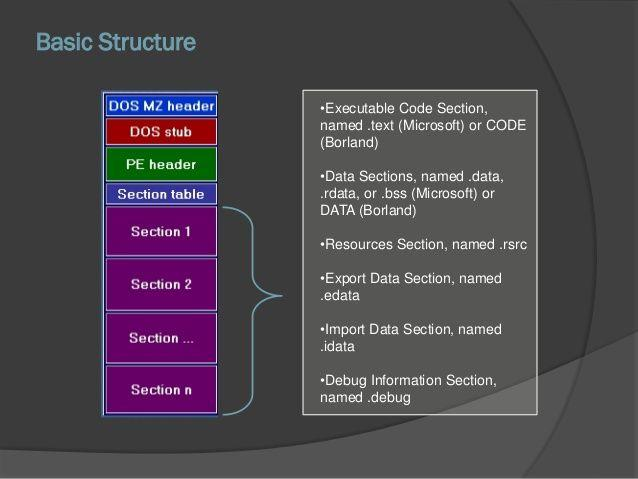
\includegraphics[scale=0.5]{images/pe_header.jpg}
    \caption{Structure PE}
    \label{structure_pe}
\end{figure}

    \subsubsection{En-tête MZ-DOS}
    Tout fichier PE doit commencer par l'en-tête \emph{MZ-DOS}. Cet en-tête permet au système d'exploitation, au 
    moment de l'exécution d'un fichier de reconnaître si c'est un exécutable valide ou non. \cite{pe2} %vérifié

    \subsubsection{En-tête PE}
    Cet en-tête contient des champs d'information comme l'offset et la taille des zones de code et de données, 
    le système d'exploitation dont le fichier est destiné, la taille de la pile initiale et 
    d'autres informations vitales. \cite{pe3} %vérifié

    Les premiers bytes sont pris par \emph{MS-DOS stub} qui a le rôle d'afficher un message d'erreur en cas ou 
    l'exécutable est lancé dans un environnement qui ne supporte pas \emph{Win32}, les bytes suivants constituent 
    une structure de données appelée \emph{\textsc{image\_nt\_headers}} dont les champs sont : %vérifié
    \begin{description}
        \item[image\_file\_header :] C'est une structure contenant les informations nécessaires
            sur le fichier comme le nombre de sections, le processeur à qui le fichier est destiné \ldots etc. %vérifié
        \item[image\_optional\_header :] C'est une structure contenant des informations cruciales comme l'adresse
            du point d'entré. %vérifié
    \end{description}

    \subsubsection{Les sections}
    Tous codes, données et ressources sont stockés dans les sections. Une section se compose de deux 
    parties : une partie en-tête et une autre pour les données. Chaque en-tête est d'une longueur de 40 
    bytes ; il contient le nom de la section, la taille des données, l'offset de la section dans 
    le ficher PE, et l'adresse de début de la plage d'adresse du processus courant où la section doit être 
    chargée. \cite{pe4}

\section{Conclusion}
À la fin de ce chapitre, des notions plus ou moins poussées concernant les virus --- comme les méthodes d'infections 
et les méthodes de dissimulation --- ont été abordées et étudiées. Ces notions sont indispensables pour cerner le 
mode de fonctionnement des virus. Ainsi que pour la mise en œuvre du projet et du prochain chapitre. %vérifié
